%% ****** Start of file template.aps ****** %
%%
%%
%%   This file is part of the APS files in the REVTeX 4 distribution.
%%   Version 4.0 of REVTeX, August 2001
%%
%%
%%   Copyright (c) 2001 The American Physical Society.
%%
%%   See the REVTeX 4 README file for restrictions and more information.
%%
%
% This is a template for producing manuscripts for use with REVTEX 4.0
% Copy this file to another name and then work on that file.
% That way, you always have this original template file to use.
%
% Group addresses by affiliation; use superscriptaddress for long
% author lists, or if there are many overlapping affiliations.
% For Phys. Rev. appearance, change preprint to twocolumn.
% Choose pra, prb, prc, prd, pre, prl, prstab, or rmp for journal
%  Add 'draft' option to mark overfull boxes with black boxes
%  Add 'showpacs' option to make PACS codes appear
%  Add 'showkeys' option to make keywords appear
\documentclass{revtex4}
%\documentclass[aps,prl,preprint,superscriptaddress]{revtex4}
%\documentclass[aps,prl,twocolumn,groupedaddress]{revtex4}
\usepackage[dvipdf]{graphicx}
%\usepackage{dcolumn}

% You should use BibTeX and apsrev.bst for references
% Choosing a journal automatically selects the correct APS
% BibTeX style file (bst file), so only uncomment the line
% below if necessary.
%\bibliographystyle{apsrev}

\begin{document}

% Use the \preprint command to place your local institutional report
% number in the upper righthand corner of the title page in preprint mode.
% Multiple \preprint commands are allowed.
% Use the 'preprintnumbers' class option to override journal defaults
% to display numbers if necessary
%\preprint{}

%Title of paper
\title{Large-Angle Motion of a Pendulum}
\vspace*{5mm}

% repeat the \author .. \affiliation  etc. as needed
% \email, \thanks, \homepage, \altaffiliation all apply to the current
% author. Explanatory text should go in the []'s, actual e-mail
% address or url should go in the {}'s for \email and \homepage.
% Please use the appropriate macro foreach each type of information

% \affiliation command applies to all authors since the last
% \affiliation command. The \affiliation command should follow the
% other information
% \affiliation can be followed by \email, \homepage, \thanks as well.
% \author{Jason P. Longacre}
%\homepage[]{Your web page}
%\thanks{}
%\altaffiliation{}
\author{Physics 2502, University of Connecticut}
%\author{R.T. Jones}
%\affiliation{University of Connecticut}

%Collaboration name if desired (requires use of superscriptaddress
%option in \documentclass). \noaffiliation is required (may also be
%used with the \author command).
%\collaboration can be followed by \email, \homepage, \thanks as well.
%\collaboration{}
%\noaffiliation

\date{\today}

\begin{abstract}
The pendulum is one of the most familiar examples of simple harmonic
motion known to students of physics, and yet it is not a truly harmonic
system, even in the case when the effects of friction are negligible.
In this experiment students measure the period of a pendulum as a function
of its amplitude, and discover that significant deviations from simple
harmonic behavior take place even for amplitudes of only a few degrees.
A rigid-rod pendulum and a photogate are used to investigate the
period of the pendulum as a function of its angular amplitude, measured
by analyzing a video taken of the pendulum motion over many periods.
These results are compared with the solution obtained by integrating the
true equation of motion for the ideal pendulum.  Deviations from ideal
behavior are investigated in terms of a model that includes both the
effects of air drag and imperfections in the pivot.
\end{abstract}

% insert suggested PACS numbers in braces on next line
%\pacs{}
% insert suggested keywords - APS authors don't need to do this
%\keywords{}

\setlength{\topmargin}{0in}

%\maketitle must follow title, authors, abstract, \pacs, and \keywords
\maketitle

% body of paper here - Use proper section commands
% References should be done using the \cite, \ref, and \label commands

%% The normal text is displayed in two-column format, but special
%% sections spanning both columns can be inserted within the page
%% format so that long equations can be displayed. Use
%% sparingly.
%%\begin{widetext}
%% put long equation here
%%\end{widetext}
%
%% figures should be put into the text as floats.
%% Use the graphics or graphicx packages (distributed with LaTeX2e)
%% and the \includegraphics macro defined in those packages.
%% See the LaTeX Graphics Companion by Michel Goosens, Sebastian Rahtz,
%% and Frank Mittelbach for instance.
%%
%% Here is an example of the general form of a figure:
%% Fill in the caption in the braces of the \caption{} command. Put the label
%% that you will use with \ref{} command in the braces of the \label{} command.
%% Use the figure* environment if the figure should span across the
%% entire page. There is no need to do explicit centering.
%
%%\begin{turnpage}
%% Surround figure environment with turnpage environment for landscape
%% figure
%% \begin{turnpage}
%% \begin{figure}
%% \includegraphics{}%
%% \caption{\label{}}
%% \end{figure}
%% \end{turnpage}
%
%% tables should appear as floats within the text
%%
%% Here is an example of the general form of a table:
%% Fill in the caption in the braces of the \caption{} command. Put the label
%% that you will use with \ref{} command in the braces of the \label{} command.
%% Insert the column specifiers (l, r, c, d, etc.) in the empty braces of the
%% \begin{tabular}{} command.
%% The ruledtabular enviroment adds doubled rules to table and sets a
%% reasonable default table settings.
%% Use the table* environment to get a full-width table in two-column
%% Add \usepackage{longtable} and the longtable (or longtable*}
%% environment for nicely formatted long tables. Or use the the [H]
%% placement option to break a long table (with less control than 
%% in longtable).
%
%
%% Surround table environment with turnpage environment for landscape
%% table
%% \begin{turnpage}
%% \begin{table}
%% \caption{\label{}}
%% \begin{ruledtabular}
%% \begin{tabular}{}
%% \end{tabular}
%% \end{ruledtabular}
%% \end{table}
%% \end{turnpage}
%
%% Specify following sections are appendices. Use \appendix* if there
%% only one appendix.
%%\appendix
%%\section{}
%

\section{Introduction}

The pendulum is perhaps the most studied mechanical system in
introductory physics laboratories. In most of these
experiments (Foucalt's pendulum, Kater's pendulum, physical
pendulum and coupled pendula) the amplitude is restricted to
small angles so that the period approximately obeys the familiar relation,
\begin{equation}
\tau_0 = 2\pi\frac{I}{mgL}
\label{eq:omega0}
\end{equation}
where $I$ is the pendulum moment of interia about the pivot, $m$ is its
mass, $L$ is the distance from the pivot to its center of mass, and $g$ is
the local acceleration of gravity.  This is actually the limiting value
of the period for small-amplitude oscillations; for oscillations of finite
amplitude there are corrections which must be applied in order to accurately
predict the period.  Although these are often called {\em large-amplitude}
corrections, their effects are present at any non-zero amplitude, and are
readily observable for oscillations as small as a degree.  The purpose of
this experiment is to measure the period of a physical pendulum as a
function of its amplitude, and compare these with the predictions based
on a model of the ideal pendulum.

\begin{figure}
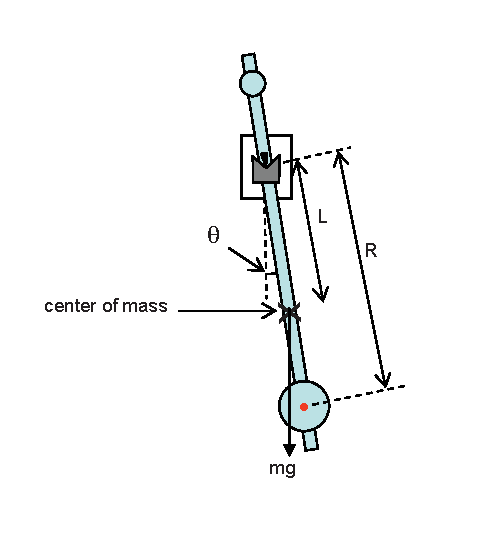
\includegraphics[width=3in]{pendu.eps}
\caption{\label{fig:pendu}
Schematic diagram of the pendulum used in this experiment. The dashed line
is the vertical which is the equilibrium position of the rod.  The length
$L$ is the distance from the pivot point to the center of mass of the 
pendulum, while $R$ is the distance from the pivot to the marker used to
track the pendulum position in the video.
}
\end{figure}

\section{Model of the Physical Pendulum}

Consider the physical pendulum depicted in Fig.~\ref{fig:pendu}.  Located
somewhere along the length of the pendulum shaft, at a distance $R$ from
the pivot, is a brightly-colored marker that facilitates
automatic tracking of the pendulum position using video analysis software.
Ignoring friction, the equation of motion for this system is
\begin{equation}
I\frac{d^2\theta}{dt^2} = -mgL \sin{\theta}
\label{eom:ideal}
\end{equation}
The small-amplitude solution to this equation of motion is
\begin{equation}
\theta(t)=\theta_0 \cos(\omega_0 t + \delta_0)\,\,
,\,\,\,\,\omega_0=\sqrt{\frac{mgL}{I}}
\label{sol:idealsa}
\end{equation}
This is not the exact solution to Eq.~\ref{eom:ideal}, but to a related
equation of motion that is obtained by replacing the factor $\sin{\theta}$
on the right-hand side of Eq.~\ref{eom:ideal} with its small-angle
approximation $\theta$.  Finding exact solutions to Eq.~\ref{eom:ideal}
is more difficult because the differential equation is non-linear, so the
solution is no longer a perfect sine wave.  However, the motion is still
periodic, repeating itself every $\tau$ seconds.  It turns out that a very
good description of the motion of a pendulum at amplitudes less than
30$^{\circ}$ is obtained using the solution Eq.~\ref{sol:idealsa}, but
with the true frequency $\omega=2\pi/\tau$ in the place of $\omega_0$.

\subsection{period of the ideal pendulum}

Unlike the value of $\omega_0$ in Eq.~\ref{sol:idealsa}, the value of
$\omega$ depends on the oscillation amplitude.  To work this out, consider
the energy carried by the pendulum during its motion.
The potential energy of the pendulum is $U=mgL(1-\cos{\theta})$ where the
zero of potential energy has been chosen to be at the equilibrium position
$\theta=0$.  The total mechanical energy of the pendulum is given by,
\begin{equation}
E= K + U = \frac{1}{2}I\dot{\theta}^2 + mgL(1-\cos{\theta}).
\label{eq:Etot}
\end{equation}
Consider now the initial condition at $t=0$ where the bob is
released from rest at an angle $\alpha$. The principle of mechanical
energy conservation requires that
\begin{equation}
mgL(1-\cos{\alpha}) = \frac{1}{2}I\dot{\theta}^2 + mgL(1-\cos{\theta})
\label{eq:Econs}
\end{equation}
Rearranging Eq.~\ref{eq:Econs} and taking a square root, the angular
velocity of the pendulum is
\begin{equation}
\dot{\theta} = \sqrt{2\omega_0^2(\cos{\theta} - \cos{\alpha})}
\label{eq:thetadot}
\end{equation}
Using the identity, $\cos{\alpha}= 1-2\sin^2{\alpha/2}$,
Eq.~\ref{eq:thetadot} can be written as
\begin{equation}
\frac{d\theta}{dt}=2\omega_0\sqrt{\sin^2{\alpha/2}-\sin^2{\theta/2}}
\label{eq:dthetadt}
\end{equation}
This equation can then be integrated from 0 to $\alpha$ which is
the quarter-period time interval t=0 to $\tau/4$.  The result is
\begin{equation}
\tau = \frac{2}{\omega_0}\int_0^{\alpha}{\frac{d\theta}
{\sqrt{\sin^2{\alpha/2}-\sin^2{\theta/2}}}}
\label{eq:tau}
\end{equation}

There are two features about Eq.~\ref{eq:tau} which are quite unpleasant.
Note first that the integral is improper since the integrand is undefined
(infinite) when $\theta=\alpha$ at the upper limit. Extreme care must be
taken when numerically evaluating such improper integrals.
The second point is that the form of Eq.~\ref{eq:tau} obscures the
fact that, for small $\alpha$, it approaches the simple result of
Eq.~\ref{eom:ideal}, independent of amplitude $\alpha$.  To help with the
second problem, consider a change of variables from $\theta$ to $\phi$
defined as
\begin{equation}
\sin{\phi}=\frac{\sin{\theta/2}}{\sin{\alpha/2}}
\label{eq:phi}
\end{equation}
such that $\phi$ advances from 0 to $2\pi$ during one
full oscillation of the pendulum.  Eq.~\ref{eq:phi} can be used to
rewrite Eq.~\ref{eq:tau} as
\begin{equation}
\frac{\tau}{\tau_0} = \frac{2}{\pi}\int_0^{\frac{\pi}{2}}{\frac{d\phi}
{\sqrt{1-k^2\sin^2{\phi}}}}
\label{eq:tauovertau0}
\end{equation}
where $k=\sin{\alpha/2}$.  Using Eq.~\ref{eq:tauovertau0}
makes it is easy to see that $\tau\rightarrow\tau_0$ in the limit
$k\rightarrow 0$, which corresponds to $\alpha\rightarrow 0$.

For non-zero $k$, one must evaluate this integral, which is a member of
a special class known as ``elliptic integrals''.  Since this is a definite
integral, it can be evaluated numerically and expanded in a power series
in the free parameter $k$.  The solution is
\begin{equation}
\frac{\tau}{\tau_0} = 1 + \left(\frac{1}{2}\right)^2k^2
+ \left(\frac{1\cdot 3}{2\cdot 4}\right)^2k^4
+ \left(\frac{1\cdot 3\cdot 5}{2\cdot 4\cdot 6}\right)^2k^6
+ \cdots
\label{eq:tauofk}
\end{equation}
which is convergent as long as $k<1$.

\subsection{including effects of friction}

Thus far it has been assumed that the mechanical energy $E$ is a constant
of the pendulum's motion.  This assumption is violated by the presence of
dissipative forces, both in the form of the drag produced by the viscosity
of the air through which the pendulum moves, and also by the contact
friction created as the pivot rotates in the support groove.
Both of these effects can be incorporated into the simple harmonic model
of the small-oscillation pendulum.

Incorporating air drag into the model leads to the following modifications
to Eq.~\ref{eom:ideal},
\begin{equation}
I\frac{d^2\theta}{dt^2} = -mgL \sin{\theta} -b\frac{d\theta}{dt}
\label{eom:real}
\end{equation}
The drag coefficient $b$ sets the scale for the torque produced by the
drag force.  Solving Eq.~\ref{eom:real} leads to the familiar damped
oscillator solutions, with the exact form depending on whether $b$ is
small (under-damped), large (over-damped), or in between (critically damped).
In this experiment the value of $b$ is small enough that the scale of the
drag torque is much smaller than the scale of the gravitational torque,
so the under-damped solution is the appropriate one.
\begin{equation}
\theta(t)=\theta_0 e^{-\Gamma t} \cos(\omega t + \delta_0)\,\,
,\,\,\,\,\Gamma=\frac{b}{2I}
\label{sol:damped}
\end{equation}
As explained above, this is only an exact solution to Eq.~\ref{eom:real}
in the limit of small oscillations, but using the true frequency $\omega$
obtained in the previous section in the place of the small-oscillation
frequency $\omega_0$ allows this solution to work very well at amplitudes
as large as 30$^{\circ}$.

The pivot is designed to have a very small a frictional torque, but at very
small amplitudes it can be comparable to the torque from air drag.  Its
small magnitude allows us to treat contact friction as a small perturbation
to the motion described by Eq.~\ref{sol:damped}.  Kinetic friction produces
an approximately constant torque, independent of velocity, that opposes the
direction of the swing.  Inserting a small constant torque into
Eq.~\ref{eom:real} causes the equilibrium position of the pendulum to be
displaced by a miniscule amount away from $\theta=0$.  Because the friction
force always opposes the direction of the motion, this displacement reverses
sign each time the pendulum reverses direction.  This does not affect the
period of the pendulum, but it causes the pendulum to lose a little bit of
amplitude upon each half-swing.  One way to calculate the damping effect
from friction in the mount is to compute the work $\Delta W_f$ done by the
pendulum against friction during each period
\begin{equation}
\Delta W_f = -\mu_k m g (2r\alpha)
\label{eq:workf}
\end{equation}
where $r$ is the distance from the contact point to the center of rotation
in the pivot, and $2\alpha$ is the total angular distance travelled by the
pendulum during between one complete period.  The important thing to 
note here is not the exact value of $\Delta W$ but how it is proportional
to the oscillation amplitude $\alpha$.  By contrast, the work done by the
drag force in Eq.~\ref{eom:real} during one period,
\begin{eqnarray}
\Delta W_d &=& -b\int_0^{\tau}{\frac{d\theta}{dt}d\theta} \nonumber \\
&=& -\frac{\pi b \omega}{2} \alpha^2
\label{eq:workd}
\end{eqnarray}
is proportional to the square of the amplitude $\alpha$.  Because of this,
drag forces tend to dominate the damping at larger oscillation amplitudes,
while pivot friction becomes important at small amplitudes, and causes the
damping coefficient $\Gamma$ in Eq.~\ref{sol:damped} to increase somewhat
at very small amplitudes.  Other than this, the effects of kinetic friction
on the motion are essentially the same as the drag force, causing the
amplitude of the motion to decrease exponentially.  It can be 
incorporated into Eq.~\ref{sol:damped} by making $\Gamma$ weakly dependent
on the amplitude, increasing somewhat at very small amplitudes.  For the
purposes of this experiment, treating $\Gamma$ as a constant is a very good
approximation.

\subsection{imperfections in the mount}

Empirically one finds that the oscillation period of a pendulum like the
one used in this experiment decreases faster at low amplitude than is
predicted by Eq.~\ref{eq:tauofk}.  The explanation for this comes from
mechanical imperfections in the mount.  In the ideal case, viewing the
knife edge of the pendulum pivot under a microscope would reveal that the
edge is actually rounded in the form of a half-cylinder with a uniform
radius $r$ that rolls back and forth on a small flat section at the base
of the groove in the mount.  Small burrs on this surface, which accumulate
with use of the apparatus as the pendulum is unmounted and remounted during
experiments, as well as general wear of the surface on which it rocks back
and forth, distort the geometry from this ideal shape.  These distortions
can result in multiple contact points around the tip of the knife edge
that the pivot rides up onto as it rocks back and forth during oscillations,
all of which are within $\pm r$ of the center of the knife edge.  For a
crude model of this, consider a knife edge that has been distorted into
a square shape, with two corners a distance $2r$ apart sitting on a flat
supporting surface.  As the pendulum swings right, it rises up onto the
left corner a displacement $-r$ from the center of the pivot, and as the
pendulum swings back left of center, it switches over and rocks up on the
right corner at $+r$.  This is just a distortion of
the shape of the gravitational potential curve of the pendulum, and does
not involve friction, so it cannot result in energy loss of damping.
Instead, it causes the oscillation period to decrease by $\Delta\tau$ from
the ideal value given in Eq.~\ref{eq:tauofk}.
\begin{equation}
\Delta\tau = -\left(\frac{2r}{\pi L\alpha}\right) \tau
\label{eq:deltatau}
\end{equation}
Note that the diameter $2r$ of the knife edge is typically of order
10$^{-4}$~m, while $L$ is of order 1~m, so this frequency shift is only
significant for amplitudes $\alpha$ less than 0.1~radians.  This effect
is seen in Fig.~\ref{fig:penduap}, which shows actual measurements of the
measured period vs.\ amplitude taken with an apparatus
similar to the one used for this experiment.  The red curve shows the
prediction based on Eq.~\ref{eq:tauofk}.  The heavy solid lines are
measurements, and the dashed line passing through them is an empirical
interpolation of those data, including a term proportional to $-1/\alpha$
that causes the period to turn downward at small amplitudes.

At large amplitudes there is a related effect in the pivot that again
causes the measured period to decrease relative to that of the ideal
pendulum.  When the pendulum angle increases above a certain point, the
sides of the knife edge in the pivot begin to make contact with the
sides of the groove in the support.  This induces a new restoring torque
that acts in addition to gravity, causing the period to decrease relative
to the ideal case assumed in Eq.~\ref{eq:tauofk}.  This effect is seen
in Fig.~\ref{fig:penduap} at amplitudes above 0.3 radians, where the
measured period falls below the curve for the ideal pendulum.  For an
apparatus similar to the one used to produce Fig.~\ref{fig:penduap},
the range of near-ideal behavior is seen to lie between 0.1 and 0.25
radians.

\begin{figure}
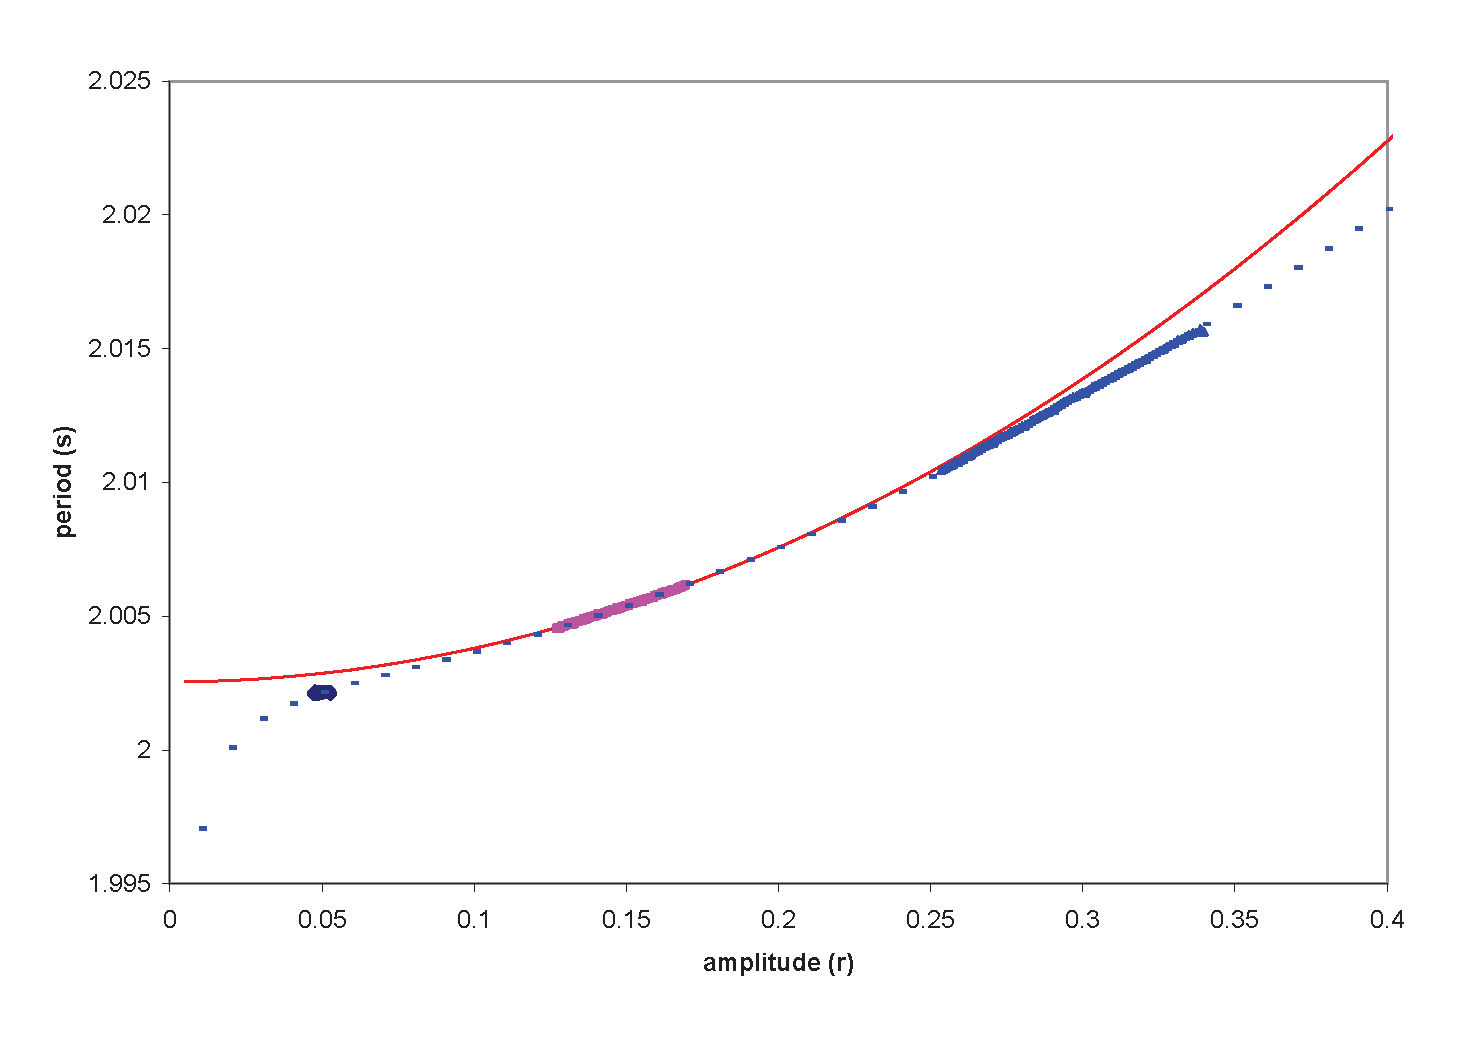
\includegraphics[width=6in]{penduap.eps}
\caption{\label{fig:penduap}
Plot of the measured period of an apparatus similar to the one used in
this experiment, as a function of oscillation amplitude.  The red curve
is the theoretical prediction based on Eq.~\ref{eq:tauofk}.  The heavy
solid lines are measurements, and the dashed line is an interpolation
of the measurements over the full dynamic range of the pendulum.
}
\end{figure}

\section{Experimental Method}

The setup used in this experiment is shown in Fig.~\ref{fig:pendu}.
At the bottom of its motion, the pendulum passes through a photogate
sensor that sends a signal to the data acquisition computer each time
the light signal is interrupted.  Measure the distance $R$ from the
suspension point to the center of the marker that will be used to
track the position of the pendulum throughout its swing.  Measure this
distance several times, and try to obtain an accuracy of $\pm 1$~mm.

Mount the pendulum on the pivot and start it swinging with a few-degree
amplitude.  On the data acquisiton computer, start the photogate program.
In the program graphical window, change the minimum and maximum period
values to reasonable values like 0.5 and 5.0 seconds and set the total
number of periods to 90, then press GO.  The program displays the time
interval between each photogate pulse, which is a half-period when the
photogate is aligned with the equilibrium position of the pendulum.
Carefully slide the photogate back and forth (taking care not to move
the arms of the photogate into the path of the pendulum) until the two
half-periods are approximately equal.  A 1\% difference is ok.

Set up the video camera and align it so that it is viewing the pendulum
along a line of sight that is perpendicular to the plane of the pendulum
motion and that passes through the pendulum marker when it is in the
equilibrium position.  Check that the field of view in the camera is
large enough that the marker never goes out of view, even when the amplitude
is the largest allowed, typically around 30$^{\circ}$.  Set the camera to
record video at medium resolution (640 x 320 is good).  The frame rate
should be between at least 30~fps.  Higher frame rates are permitted, but
will result in larger video files.

Place an object with distance markings (a meter stick is ideal) in the
view of the camera just behind the pendulum.  This will be useful later
on for calibrating the distance scale in the video.  Level the calibration
object so that at edge is clearly visible to define the horizontal axis.
Try to arrange the stand for the photogate so that the pendulum marker
is visible to the camera at all points during its swing.
When everything is aligned, start the data acquisition program and the
video recording when the pendulum is at rest.

Based on the period vs.\ amplitude curve shown in Fig.~\ref{fig:penduap},
chose three starting amplitudes within the region between 0.1 radians
and 0.25 radians.  Manually raise the pendulum to its maximum amplitude
near 15$^{\circ}$.  After a pause, release the pendulum and allow it to
swing freely, recording video and period data for a total of 90 periods.
When the data acquisition finishes, enter a descriptive name for the
data file and save it.  Stop the video recording and save the video file.
This gives about 3 minutes of video, which produces a reasonably small
file that can be easily transfered from the camera to the data acquisition
computer.  Save the file together with the period data file, using names
that clearly identify them as going together.

Repeat the above measurements for a series of successively smaller initial
amplitude values, until the final set has an amplitude of about 6-7~cm.  A
total of 3 or 4 runs is sufficient.

\section{Video Analysis}

\begin{figure}
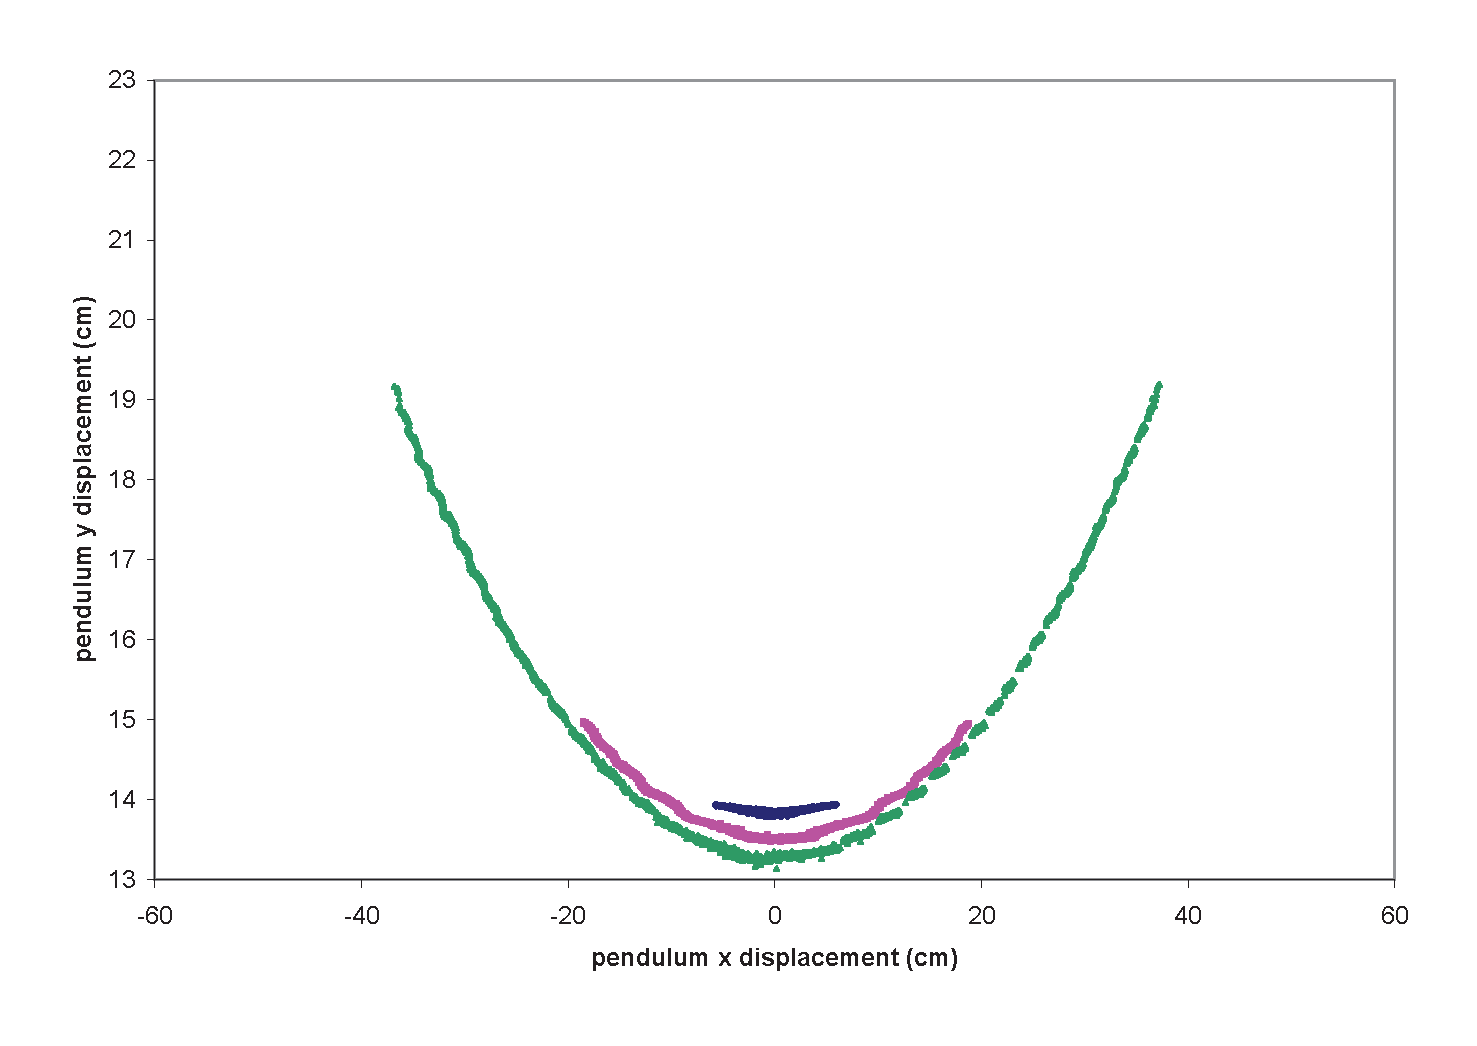
\includegraphics[width=6in]{penduxy.eps}
\caption{\label{fig:penduxy}
Plot of the position measurements of the pendulum marker, for the data
shown in Fig.~\ref{fig:penduap}.  Note that the apex of the curves are
all centered at $x=0$ and the maximum limits in $y$ for each curve are
left-right symmetric, showing that the axis alignment is correct.
}
\end{figure}

The video analysis should be carried out in the laboratory
period, so that the video data does not need to be carried away by each
student.  Stop the photogate program on the data acquisition computer, and
start the {\em Tracker}\cite{trackerprog}
video analysis program.  Open the first video file.
The first frame of the video should appear in the window.  Use the slider
at the bottom of the video screen to advance the video to where you can see
the hand releasing the pendulum, then step forward frame-by-frame until the
person is out of the view and the pendulum has reached the maximum height.
Record the frame number as the start frame.  Now press the button at the
lower right corner of the screen called ``clip settings'', and enter the
start frame number.  Leave the end frame unchanged, and press OK.  Move the
frame slider back to the start frame.  Select menu item {\em Tracks}
$\rightarrow$ {\em New} $\rightarrow$ {\em Point Mass}.  Right-click on
the new button just created in the {\em Mass Control} menu, and select
{\em Autotracker}.  This brings up the Autotracker wizard tool.  First
the program wants you to select the pendulum marker in the video.  Center
the loop cursor on the marker in the video and left-click.  You can now
resize and reposition the target image to optimize image recognition.  After
this you select the size and position of the search box in which the
autotracker looks for the marker.  The search box should be large enough
that the box centered on the marker in frame $n$ will always contain the
marker image in frame $n+1$.  Smaller search boxes make analysis faster,
so try several settings here until the optimum is found.  The autotracker
supports a feature called ``look-ahead'', which causes it to try and
extrapolate forward from previous points where it thinks the marker will
be, and center the search box there.  Running with this enabled can allow
you to use a smaller search box, but generally the tracking is more stable
with it turned off.

Allow the autotracker to analyze the entire clip.  This can take a while.
You can monitor its progress by watching the frame number change in the
autotracker control window.  If it fails to find the marker in any frame,
it will stop and give you a change to reposition the search window, or
skip that frame.  Skipping a few frames will have negligible effect on
the quality of your results.

Before you save the results, you should first include some calibration data.
Slide the frame slider back to frame 1, when the pendulum was at rest.
Select the tape measure tool from the toolbar (looks like a double-arrow
line with a number next to it) and click on the image to add it.  Click
on the two ends of the arrow, one at a time, and drag them to the two ends
of the meter stick (or other distance reference) in the image.  Click on
the number above the arrow and enter the true distance in cm.  Record the
angle of the horizontal line in the image (displayed just below the toolbar).
Next select the axis cross-hairs tool from the toolbar, and place axes on
the picture.  Click on the origin of the cross-hairs and move them to the
rest position of the marker.  Enter the angle recorded above into the box
for the axis angle.  Check that the vertical axis aligns with the pendulum
rod, confirming that the horizontal and vertical axes are perpendicular in
the video.  If this is not the case, it indicates problems with your camera
alignment.  Save the results to disk, using the same file name as the
video.  A new file with the extension {\em .trk} is created.

Open the {\em .trk} file in a browser.  With a little work, you should
be able to find the coordinate origin and axis rotation angles recorded
in video pixel units.  The time interval $\Delta t$ between frames is
recorded in the file as {\em delta\_t}.  Open a new spreadsheet and create
columns $t$, $u$, and $v$.  Extract the tracker coordinates recorded in
the file as $x$ and $y$ values, and enter them into the spreadsheet as
$u$ and $v$.  There will be several thousand of these, so do not attempt
to do this manually.  See the TA if you need help finding tools to do
this extraction.  Create new rows at the top of the spreadsheet to hold
calibration data for the coordinates of the origin $u_0$ and $v_0$, the
scale factors $S_u$ and $S_v$, and the rotation angle $\beta$.  Create
new columns next to those for $u$ and $v$ and label them $x$ and $y$,
filling them according to the linear transformation
\begin{eqnarray}
x &=& (u-u_0)S_u\cos\beta + (v-v_0)S_v\sin\beta \nonumber \\
y &=& -(u-u_0)S_u\sin\beta + (v-v_0)S_v\cos\beta \nonumber
\end{eqnarray}
Apply this tranformation to the entire columns of data, then convert
the $x$ and $y$ values to $\theta$ through the equation
\begin{equation}
\theta = \tan^{-1}\left(\frac{x}{R-y}\right)
\end{equation}
Finally, fill in the values in the $t$ column, starting at 0 in the first
row of the table and increasing by $\delta t$ going down the column.
Save the spreadsheet to disk frequency to prevent loss of your work.

Within the spreadsheet, create duplicates of the first worksheet, copying
all of the data and formulas.  Rename the worksheets, one for each of your
video runs.  Repeat the above video analysis for each of your videos.
Extract the data from each of the {\em .trk} files and overwrite the
calibration and $u,v$ columns on worksheets 2-$n$ with the corresponding
data from the files.  The formulas on these worksheets will automatically
carry out the transformations and produce the $\theta$ values.  Plots of
$y$ vs.\ $x$ should look similar to Fig.~\ref{fig:penduxy}, except that
the small and large oscillation amplitudes should be less extreme than 
the ones shown in the example.

Save this spreadsheet together with the period data files collected earlier.
Each student should carry away copies of these files for further data analysis.

\section{Data Analysis}

The challenge of data analysis for this experiment is to match up the
amplitude information extracted from the video with the period information
collected by the photogate program, so that the period can be plotted as
a function of amplitude.  This is not a simple task because the period
measurements are taken only once per period, while the amplitude information
is in the local maxima and minima that appear the oscillating function
$\theta(t)$ that was sampled once per camera frame, typically 30 or 60
times per second.  One way to proceed would be to manually scroll down
through the $\theta$ column, find the maximum and minimum amplitude for
each period, subtract them and divide by 2, and record the result as the
amplitude for that period.  Actually carrying out the analysis this way
would be exhausting however, because there are 90 periods in each data
sets, and several data sets to analyze.  A much more convenient and
powerful technique called {\em a linear filter} can be used to accomplish
the same thing in an automated fashion.  Not only is the linear filter a
much more efficient method than manual inspection, but it actually produces
amplitude estimates that are more precise than inspection could produce.

The theoretical basis for the linear filter to be used in this analysis is
presented in Appendix~\ref{app:filters}.  The emphasis here is not why it
works, but how to use it.  Think of the filter as an operator that takes
in one column $S$ of a spreadsheet as input and produces a new column $A$
of the same length as output, where $A$ contains the amplitude of the
oscillating function $S$.  The basic formula for the filter is
\begin{equation}
A_m = \sum_{n=0}^{N-1} S_{m+n} f_n
\label{eq:filter}
\end{equation}
where the numbers $f_1\cdots f_{N-1}$ are the $N$ values of the filter
column vector $f$.  In the current analysis task, the column of $\theta(t)$
values serves as the input vector $S$.  The filter vector $f$ needed for
this purpose is actually column of $N$ complex numbers.  According to
Eq.~\ref{eq:filter}, if the numbers $f_n$ are complex then this implies
that the outputs $A$ are also complex.  For the purposes of a spreadsheet
application that deals only with real numbers, Eq.~\ref{eq:filter} is can
be rewritten as,
\begin{eqnarray}
\Re{A}_m &=& \sum_{n=0}^{N-1} S_{m+n} \Re{f}_n \nonumber \\
\Im{A}_m &=& \sum_{n=0}^{N-1} S_{m+n} \Im{f}_n \nonumber \\
Amag_m &=& |A_m| = \sqrt{\Re{A}_m^2 + \Im{A}_m^2}
\label{eq:AA}
\end{eqnarray}
where $Amag_m$ stands for the absolute magnitude of
the complex number $A_m$.

Before these formulas can be implemented, one must first create concrete
instances of the filter functions $\Re{f}_n$ and $\Re{fI}_n$. 
Let us define the $N$ complex numbers $f_n$ as,
\begin{equation}
f_n = \frac{2}{N}\,e^{2\pi i\frac{n}{N}}
\label{eq:fdef}
\end{equation}
with $n=0\cdots N-1$.  With this definition, the column $\Re{f}_0\cdots
\Re{f}_{N-1}$ and $\Im{f}_0\cdots \Im{f}_{N-1}$
contain cosine and sine functions, respectively
sampled at $N$ equal intervals between 0 and $2\pi$.  In your spreadsheet,
create two new columns to the right of the $t$ column created above, and
label them ``fR filter'' and ``fI filter''.  Underneath each, create formulas
to implement Eq.~\ref{eq:fdef} that extend down just $N$ cells from the top.
Adjust your choice of $N$ so that the oscillations in the filter match the
oscillations in $\theta(t)$ as close as possible.  $N$ has to be an integer,
so the match cannot be exact, but the closer the better.  To the right of
the filter columns, create a new column called ``amplitude'', and enter a
formula to compute $Amag_m$ from Eq.~\ref{eq:AA} in it.  With Microsoft Excel,
$Amag_m$ can be computed in only one step by making use of the special function
{\tt SUMPRODUCT}.  Plot the resulting column $Amag$ vs.\ $t$ in a graph
together with the input column $\theta$ vs.\ $t$, and verify that the
results in the amplitude column agree with what you would have gotten
by taking the peak heights for each period and connecting them by a
continuous smooth curve.

Now that you have extracted the amplitude from the oscillating function,
you would like to sample the amplitude function once per period, to be
able to match it up row-for-row with the periods measured using the
photogate.  The most straight-forward way to do this is to fit the
amplitude function to a simple polynomial function, then enter the
polynomial formula into a new ``S amplitude'' column along-side the
photogate period data.  The amplitude is a smooth and slowly decreasing
function, so a second-order polynomial should give an excellent fit.
Create 3 cells in the upper portion of your worksheet to contain the
3 parameters of a second-order polynomial, and create a new column to
the right of the $Amag$ column, called ``amplitude fit'' to contain the
fit function values.  After the ``amplitude fit'' column add one for
``amplitude residuals'' and enter the usual formula for the squared
difference between the $Amag$ data and ``amplitude fit'' functions
divided by the square of the error that you assign based on fluctuations
that you observe the $Amag$ values in neighboring cells.  Up near the
parameters list, add a cell for chi-squared and its degrees of freedom.
Enter a formula for the sum of residuals in the chi-squared cell, and
use the Solver to find the best-fit values for the polynomial coefficients.
Do this for each of the amplitude data sets you collected.

Now you are ready to combine the amplitudes extracted from the video with
the periods measured using the photogate.  Find the photogate period data
contained in plain text files saved by the photogate program.
Add two new column to the right of the existing table, and name them
``t photogate'' and ``$\tau$ photogate''.   Import the period values from
the file produced by the photogate program into the ``$\tau$ photogate''
column.  There should be about 90 rows in this column at this point.
Find the extra-long period that coincides with the start of free 
oscillations, and assign the value of zero to $t photogate$ for that
cell.  Erase all of the period data from the spreadsheet before that point.
For all of the ``t photogate'' cells below the first one, insert the
formula adding the value of the ``photogate period'' in the preceeding
row to the preceeding ``t photogate''.  This produces a cummulative sum
of the measured periods ``$\tau$ photogate'' in the ``t photogate'' column.
Add a new column to the right of ``$\tau$ photogate'' called
''amplitude from fit'' and enter the polynomial formula from the fit
performed above, to compute the amplitude for the time ``t photogate'', 
based on the fit to the camera video data for this run.

Create a graph of the measured ``$\tau$ photogate'' values vs.\ 
``amplitude from fit''.  Include data from all of your runs in the same
plot.  The resulting plot should look similar to the one shown in
Fig.~\ref{fig:penduap}.  Add vertical error bars to the data points in
the plot that represent your best estimate for the errors in the photogate
period data.  You can estimate these by looking at sequential numbers in
a measured sequence, and noting the size of the random fluctuations
between consecutive measurements.  Add a curve to the plot that
represents the function $\tau(\alpha)$ in Eq.~\ref{eq:tauofk}.  To get
a good description of your data, you will need to adjust the value of
the unknown parameter $\tau_0$ in Eq.~\ref{eq:tauofk} to minimize the
chi-square between the curve and the data points with their errors.

Use a chi-square test to make a quantitative comparison between your data
and Eq.~\ref{eq:tauofk}.  If there are systematic deviations between the
data and the curve in some ranges of amplitude, as seen in 
Fig.~\ref{fig:penduap}, comment on what effects contribute to these
deviations, and repeat the chi-square test, including only data within
a restricted amplitude range where the effects of these distortions
are small.  Study the effects of each of the higher-order terms in 
Eq.~\ref{eq:tauofk} in influencing the quality of the fit.

\begin{acknowledgments}
This write-up was written by Prof. Richard Jones, based on an earlier
laboratory described by Prof. Doug Hamilton that studied the large-angle
motion of a bifilar pendulum, with periods measured using a stop-watch (1988),
and later a photogate (2004).
\end{acknowledgments}

%% Create the reference section using BibTeX:
%\bibliography{revtex4}

\begin{thebibliography}{9}

\bibitem{trackerprog}
Douglas Brown, Open Source Physics project, Tracker video analysis
program, v. 3.10, available for download at
\url{http://www.cabrillo.edu/~dbrown/tracker/}, Jan. 20, 2011.

\end{thebibliography}

\appendix
\section{Basics of Linear Filters}
\label{app:filters}
\setcounter{figure}{0}
\renewcommand*\thefigure{\Alph{section}.\arabic{figure}}

Consider a periodic function $S(t)$ with period $\tau$ such that
$S(t+\tau)=S(t)$ for all $t$.  Fourier's theorem states that $S$ can
be written in terms of its Fourier expansion as
\begin{equation}
S(t)=\sum_{p=0}^{\infty}{a_p \cos(p\omega t)}+
\sum_{n=p}^{\infty}{b_p \sin(p\omega t)}
\,\,,\,\,\,\,
\omega=\frac{2\pi}{\tau}
\label{eq:fourierex}
\end{equation}
where $a_n$ and $b_n$ indicate the amplitude and phase of the component
in $S$ that oscillates at frequency $n\omega$.  Often in experiments the
functional form of $S(t)$ is not known, but it is sampled at regular
intervals $\Delta t$, so that what one knows about $S$ is contained in the
list of values $S(t_0), S(t_1), S(t_2),\ldots$ where $t_{n+1}=t_n+\Delta t$.
Let us define a linear filter as an operator which acts on the $S_n$ to
produce a new list of numbers $A_n$ as follows,
\begin{equation}
A_m = \frac{2}{N}\sum_{n=0}^{N-1}{S_{m+n}\cos\left(2\pi q\frac{n}{N}\right)}
\label{eq:Afilterdef}
\end{equation}
where the parameters $q$ and $N$ are properties of the filter whose meaning
is made clear below.  Substituting the Fourier expansion for $S$ into
Eq.~\ref{eq:Afilterdef}, the sum can be readily computed.
\begin{eqnarray}
A_m&=&\frac{1}{N} 
\sum_{p=0}^{\infty}
a_p\left\{{\cal S}(p,-q)
\cos\left(p\omega t_m+(p\omega N\Delta t+2\pi q)\frac{N-1}{2N}\right)
+{\cal S}(p,+q)
\cos\left(p\omega t_m+(p\omega N\Delta t-2\pi q)\frac{N-1}{2N}\right)
\right\}\nonumber\\
&+&\frac{1}{N} 
\sum_{p=0}^{\infty}
b_p\left\{{\cal S}(p,-q)
\sin\left(p\omega t_m+(p\omega N\Delta t+2\pi q)\frac{N-1}{2N}\right)
+{\cal S}(p,+q)
\sin\left(p\omega t_m+(p\omega N\Delta t-2\pi q)\frac{N-1}{2N}\right)
\right\}\nonumber\\
\label{eq:Afiltersum}
\end{eqnarray}
where
\begin{equation}
{\cal S}(p,q)=
\frac{\sin\left[\frac{p\omega N\Delta t-2\pi q}{2}\right]}
{\sin\left[\frac{p\omega N\Delta t-2\pi q}{2N}\right]}
\end{equation}
These equations simplify greatly in the special case where $\Delta t$
evenly divides $\tau$, so that it is possible to chose $N$ such that
$\tau=N\Delta_t$.  Under these conditions, the factor ${\cal S}(p,q)$
reduces to $N\delta_{pq}$ and Eq.~\ref{eq:Afiltersum} becomes
\begin{equation}
A_m=a_q\cos(q\omega t_m)+b_q\sin(q\omega t_m)
\end{equation}

Defining a similar set of sine filters,
\begin{eqnarray}
B_m&=&\frac{2}{N}\sum_{n=0}^{N-1}{S_{m+n}\sin\left(2\pi q\frac{n}{N}\right)}
\nonumber\\
&=& b_q\cos(q\omega t_m)-a_q\sin(q\omega t_m)
\label{eq:Bfilterdef}
\end{eqnarray}
one can combine the two filters together to produce
\begin{equation}
A_m^2+B_m^2=a_q^2+b_q^2
\end{equation}
That is, the sum in quadrature of the $A_m$ and $B_m$ filtered versions
of $S$ yields the squared amplitude of the $q$'th harmonic in $S$.

In practice, it is often not possible to tune the sampling interval
$\Delta t$ so that the period $\tau$ is an integer multiple of $\Delta t$.
In that case, the values of ${\cal S}(p,q)$ with $p\ne q$ are not exactly
zero, and unwanted terms in Eq.~\ref{eq:Afiltersum} bleed through the filter.
In such cases, it is often possible to detune the value of $q$ somewhat
from a whole-integer value, and suppress a particular unwanted term.
For example, consider a signal with a period of 20.1~s being sampled at
a rate of 1~Hz.  Chosing $N=20$ gives a close but imperfect match between
the filter period $N\Delta t$ and the signal period $\tau$.  Because of
this, a $q=1$ filter designed to extract the amplitude of the fundamental
harmonic picks up small contributions from other harmonics as well, due
to the off-diagonal terms in the ${\cal S}(p,q)$ matrix.  If a term
involving the off-diagonal term ${\cal S}(1,-1)$ is creating a problem,
it can be suppressed by shifting $q=1$ down to $q=0.995$.  This small
shift has a negligible effect on the leading term 
(${\cal S}(1,1)\approx {\cal S}(1,0.995)\approx 1$), but it kills the
problematic term completely because ${\cal S}(1,-0.995)=0$. 
\end{document}
%%
%% ****** End of file template.aps ******
%%

\end{document}
%%
%% ****** End of file template.aps ******
%%
